% -----------------------------------------------
% Template for ISMIR 2014
% (based on earlier ISMIR templates)
% -----------------------------------------------

\documentclass{article}
\usepackage{ismir2014,amsmath,cite}
\usepackage{graphicx}
\usepackage{url}
\usepackage{units}
\usepackage{booktabs}
\usepackage{dcolumn}

% Title.
% ------
\title{Genre-specific Key Profiles}

% Single address
% To use with only one author or several with the same address
% ---------------
%\oneauthor
% {Names should be omitted for double-blind reviewing}
% {Affiliations should be omitted for double-blind reviewing}

% Two addresses
% --------------
%\twoauthors
%  {First author} {School \\ Department}
%  {Second author} {Company \\ Address}

% Three addresses
% --------------
\threeauthors
  {First author} {Affiliation1 \\ {\tt author1@ismir.edu}}
  {Second author} {\bf Retain these fake authors in\\\bf submission to preserve the formatting}
  {Third author} {Affiliation3 \\ {\tt author3@ismir.edu}}

% Four addresses
% --------------
%\fourauthors
%  {First author} {Affiliation1 \\ {\tt author1@ismir.edu}}
%  {Second author}{Affiliation2 \\ {\tt author2@ismir.edu}}
%  {Third author} {Affiliation3 \\ {\tt author3@ismir.edu}}
%  {Fourth author} {Affiliation4 \\ {\tt author4@ismir.edu}}

\begin{document}
%
\maketitle
%
\begin{abstract}
Pitch chroma are a popular feature for many MIR tasks. Using the GTZAN data set we investigate the distributions of pitch chroma for 9 different genres, the degree to
which these genres can be identified using these distributions and different strategies for achieving key-independence; namely transposition of the chroma according to its maximum value and 12-point FFT. We find that combining pitch chroma with commonly used MFCC can lead to small increase in classification accuracy using a Support Vector Machine. Furthermore these results show that the imposing key-independence has a surprisingly small affect on performance.
\end{abstract}
%
\section{Introduction}\label{sec:introduction}
\begin{itemize}
    \item   point out usage of pitch histograms/key profiles/pitch class profiles in MIR tasks (genre classification, key detection, anything else)
    \item   plot krumanshl vs. various temperley profiles
    \item   differences between midi-derived key profiles and audio-derived \cite{purwins_new_2000, gomez_tonal_2006}
    \item   what do we want to do here: analyze the differences between audio-based key profiles between genres
    \item   how we do it: use a data set that is annotated both with genres and keys, compute/visualize differences, use MDS and classification to analyze differentiability
    \item   how might this data be of use
\end{itemize}


\section{Data set}\label{sec:dataset}
The data set used was the GTZAN collection.\footnote{\url{http://marsyas.info/download/data_sets}} While this set is old and it is clear that it has its disadvantages \cite{sturm_analysis_2012}, it is a well-known, widely-used, and, last but not least, easily available set for genre classification tasks. It consists of a collection of $1000$ song excerpts divided into ten genres: Blues, Classical, Rock, Reggae, Pop, Metal, Rock, Jazz, Country and Hip Hop. 
Key annotations for the track are publicly available.\footnote{\url{github.com/alexanderlerch/data_set}} Instances that included key modulations or with a not easily identifiable key have been omitted from the labels. For example, none of the excerpts from the Classical genre is not annotated. 
The number of annotated files therefore reflects the difficulty of unambiguously identifying the key; Table~\ref{tab:NumberOfAnnotatedDataSetEntries} gives an overview of the number of annotated files and their mode. 
\begin{table}
    \begin{center}
        \begin{tabular}{|l|l|l|l|}
        \hline
        genre & \# major & \# min & \# annotated \\
        \hline
        blues 	&3 	    &95     &98\\
        \hline
        classic &0 	    &0 	    &0\\
        \hline
        country &94 	&5 	    &99\\
        \hline
        disco 	&43 	&55 	&98\\
        \hline
        hiphop 	&13 	&68 	&81\\
        \hline
        jazz 	&52 	&27 	&79\\
        \hline
        metal 	&4 	    &89 	&93\\
        \hline
        pop 	&44 	&50 	&94\\
        \hline
        reggae 	&53 	&44 	&97\\
        \hline
        rock 	&55 	&43 	&98\\
        \hline\hline
        overall &361    &476    &837\\
        \hline
        \end{tabular}
    \end{center}
   
	\caption{Number of annotated data set entries}
	\label{tab:NumberOfAnnotatedDataSetEntries}
\end{table}
MAYBE WE DONT NEED THIS TABLE - WE COULD JUST ADD A SMALL bAR PLOT WITH THE NUMBER OF ANNOTATED FILES?

Figure \ref{fig:KeyDistributionPerGenre} gives a more detailed visualization of the key distribution per genre with the root notes sorted with respect to the circle of fifths and major modes (left) separated from minor modes (right). 
\begin{figure}
    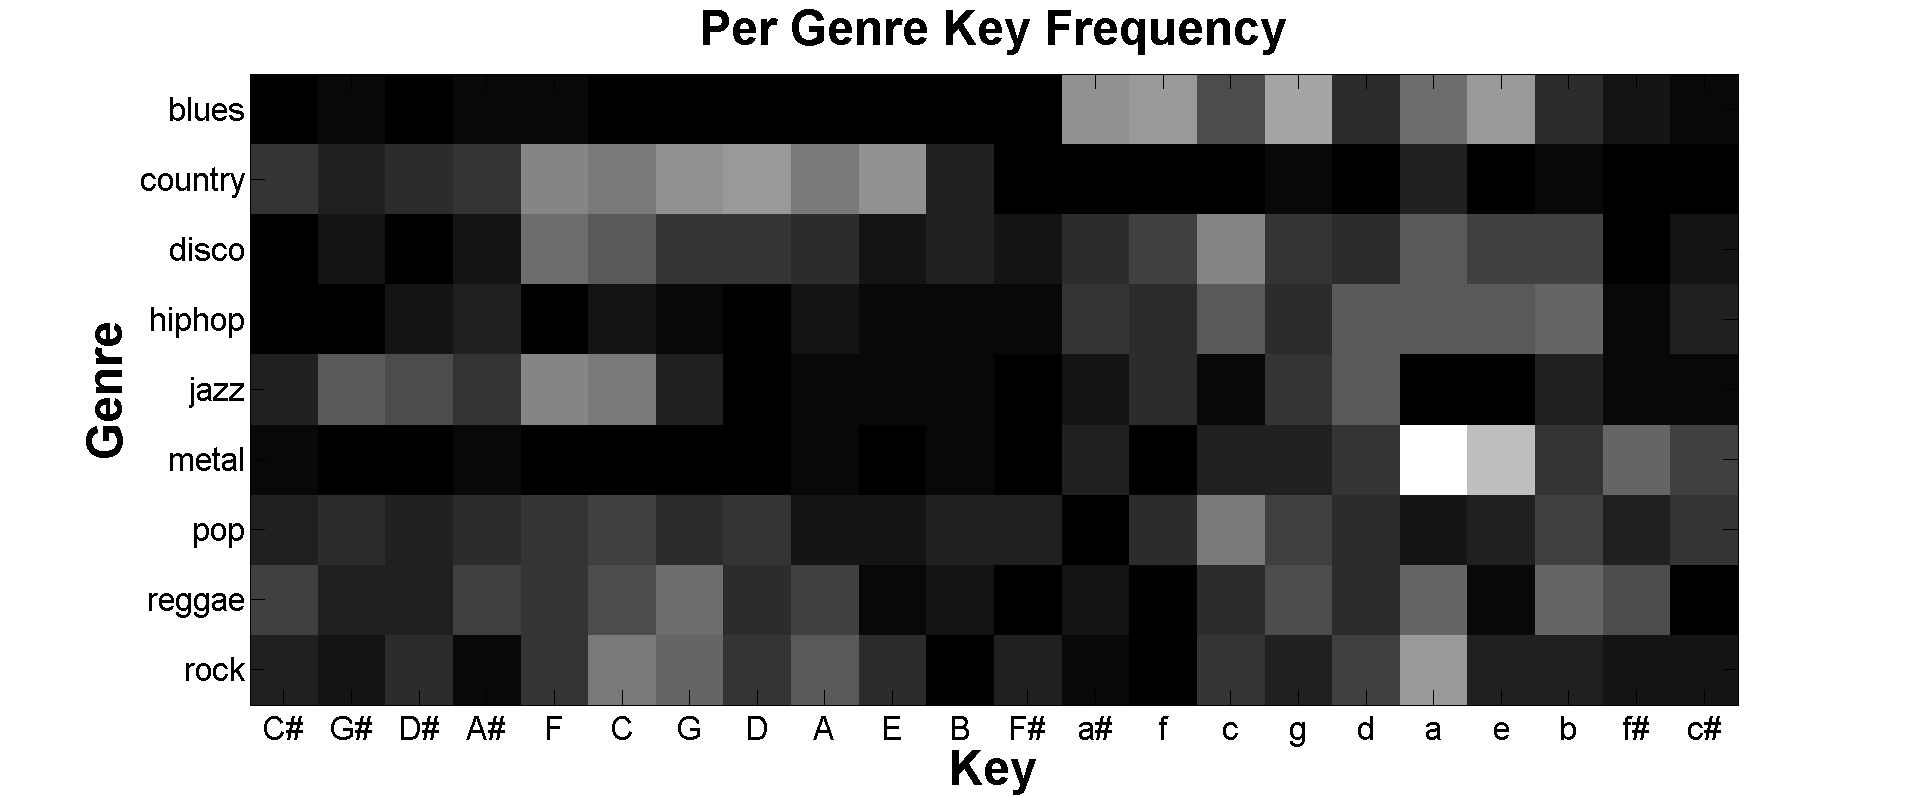
\includegraphics[scale=.2]{graph/key_distribution2}
	\caption{Key distribution per genre (brighter means more frequent) - COLOUR?}
	\label{fig:KeyDistributionPerGenre}
\end{figure}
%The distribution of keys in each genre proved unsurprising.
The relation of major vs.\ minor modes is very skewed for blues and metal (predominantly minor) as well as country (predominantly major); the genres disco, pop, reggae, and rock have a more balanced distribution between modes. Jazz tracks tend to be clustered around flat keys which are favored by trumpet and saxophone players. The keys for country cluster around C-Maj with a tendency to sharp keys. The majority of metal tracks are in either a minor or e minor, keys that are well-suited to the electric guitar and bass and correspond to the two lowest open strings. Rock is clustered around keys with few accidentals

%Pieces from the blues are mostly in the keys of G, E and B-flat. 

It is worth noting that Li and Chan presented another set of key annotations for the GTZAN data set \cite{li_genre_2011}. An examination of the two independent annotations reveals some disagreements between the two annotations: overall, about $85$ percent of the data is labeled identically. 
ICH VERSTEHE DIE ZAHLEN HIER NICHT: 67 + 119 IST DOCH MEHR ALS 15\%??
Of the differences where there was disagreement on whether a key modulation occurred or not, the majority were found in the Blues genre with 67 out 127 total disagreements of this type. If we consider only examples where both analyses agreed a modulation had \textit{not} occurred, there was a total of 119 disagreements. The most common differences were: major/relative-minor confusion (38), root/fifth confusion (35) and major/minor confusion (13).
%\begin{itemize}
    %\item   blues: $98$ vs.\ $31$ (Li) annotated tracks
    %\item   disco: $21$ differences between the two data sets
%\end{itemize}
%The genre country showed only $1$ difference. 

\section{Feature extraction}\label{sec:pitch_chroma}
We extract the key profiles per file. We use the term key profile for the overall, root-note independent pitch chroma per file. The detailed extraction is explained below.

\subsection{Pitch chroma}\label{subsec:pc_extract}
The pitch chroma is a commonly used feature in the field of Music Information Retrieval (MIR), because it is a compact, robust, and mostly timbre-independent representation of the pitch content  \cite{muller_information_2007}. It is a twelve-dimensional histogram-like octave-independent vector showing the ``strength'' of the 12 semitone classes (C, C\#, D, ..., B). It is computed by converting the spectrum to semi-tone bands and summing the energy of all bands with the distance of an octave \cite{fujishima_realtime_1999}. 
The overall pitch chroma per file is a single 12-dimensional vector that is computed by taking the median of all individual pitch chromas. 
The pitch chroma is extracted at a sample rate of \unit[10]{kHz} over a range of three octaves, starting from C at \unit[130.8]{Hz}. The FFT block size is 8192, the hop size is 4096.

 %Each track in the labeled collection was down-sampled to 10kHz and pitch chroma vectors were extracted block-wise over a three octave range, starting from C = 130.8 Hz. Pitch chroma were then normalized using the 1-norm:                     
	 %equation?
%After extracting pitch chroma for each block we can also average them over whole tracks to obtain an “averaged pitch chroma” for each track, sometimes called a Pitch Histogram [**ref]. After averaging using the median for each chroma-bin each song is then represented by a single 12-dimensional chroma vector.


\subsection{Key profiles}\label{sec:featureset}
We assume that the key profile of a song in the same mode (major or minor) should be similar between songs within one genre, but is shifted circularly to the song's root note. Under this assumption, we can ``convert'' each pitch to a key-profile by applying a circular shift to make it root-note independent. In other words, the key profile is the root note independent pitch distribution (e.g., the pitch profile of a song in A-Maj or a-min is circularly shifted by $9$ indices to the left so that the bin of pitch class A lands on the first index).

%A problem with using a pitch chroma approach is that the overall tonality of each song may dominate any between-genre differences; because the distribution of major and minor keys are not the same for each genre, songs might be classified according to their key using this method. For example pitch chroma extracted from minor tracks would be classified as Metal, since the averaged pitch chroma for Metal would be obtained by averaging pitch chroma extracted from predominantly minor tracks. This is an inherent problem in using pitch chroma as op-posed to more often used timbral features like MFCCs and in order to account for this we processed major and minor tracks separately. Another consideration revealed in the analysis of the data set is that the the key-labels are not uniformly distributed within each key. For example the majority of songs in the keys of A and E-minor are in the Rock and Metal genres. 

\section{Key Profile Analysis}
%In order to generate the key profiles for this overall analysis, we used the the KP1 key profiles.
\subsection{Overall key profiles}
Figure \ref{fig:OverallKeyProfiles} shows the overall key profiles in a box plot in comparison with other reported profiles. 
While Krumhansl's ``Probe Tone Ratings'' \cite{krumhansl_cognitive_1990} are not really a key profile (derived from listening experiments on tonality)they have been frequently used in audio key detection. They seem to correlate well with key profiles (e.g., \cite{izmirli_template_2005}). 
Temperley's key profiles are extracted from symbolic data  rather than from audio \cite{temperley_bayesian_2004,temperley_pitch-class_2008}.
\begin{figure*}[tb]
    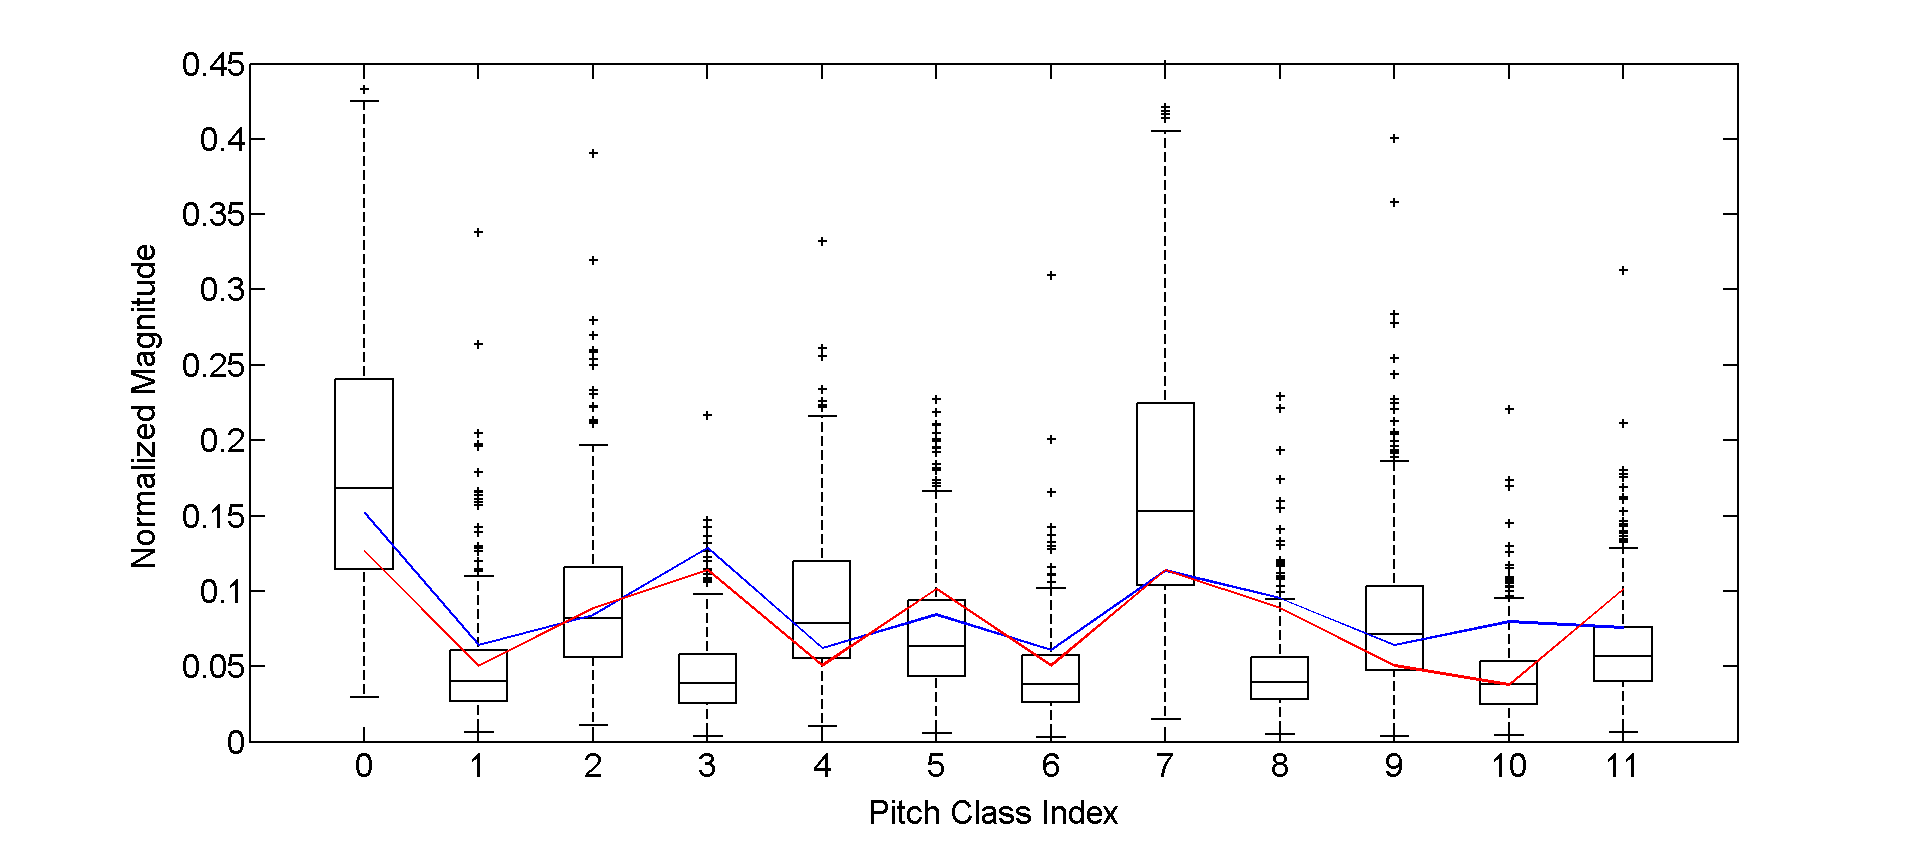
\includegraphics[scale=.2]{graph/allMajChroma+Krum+Temp}
    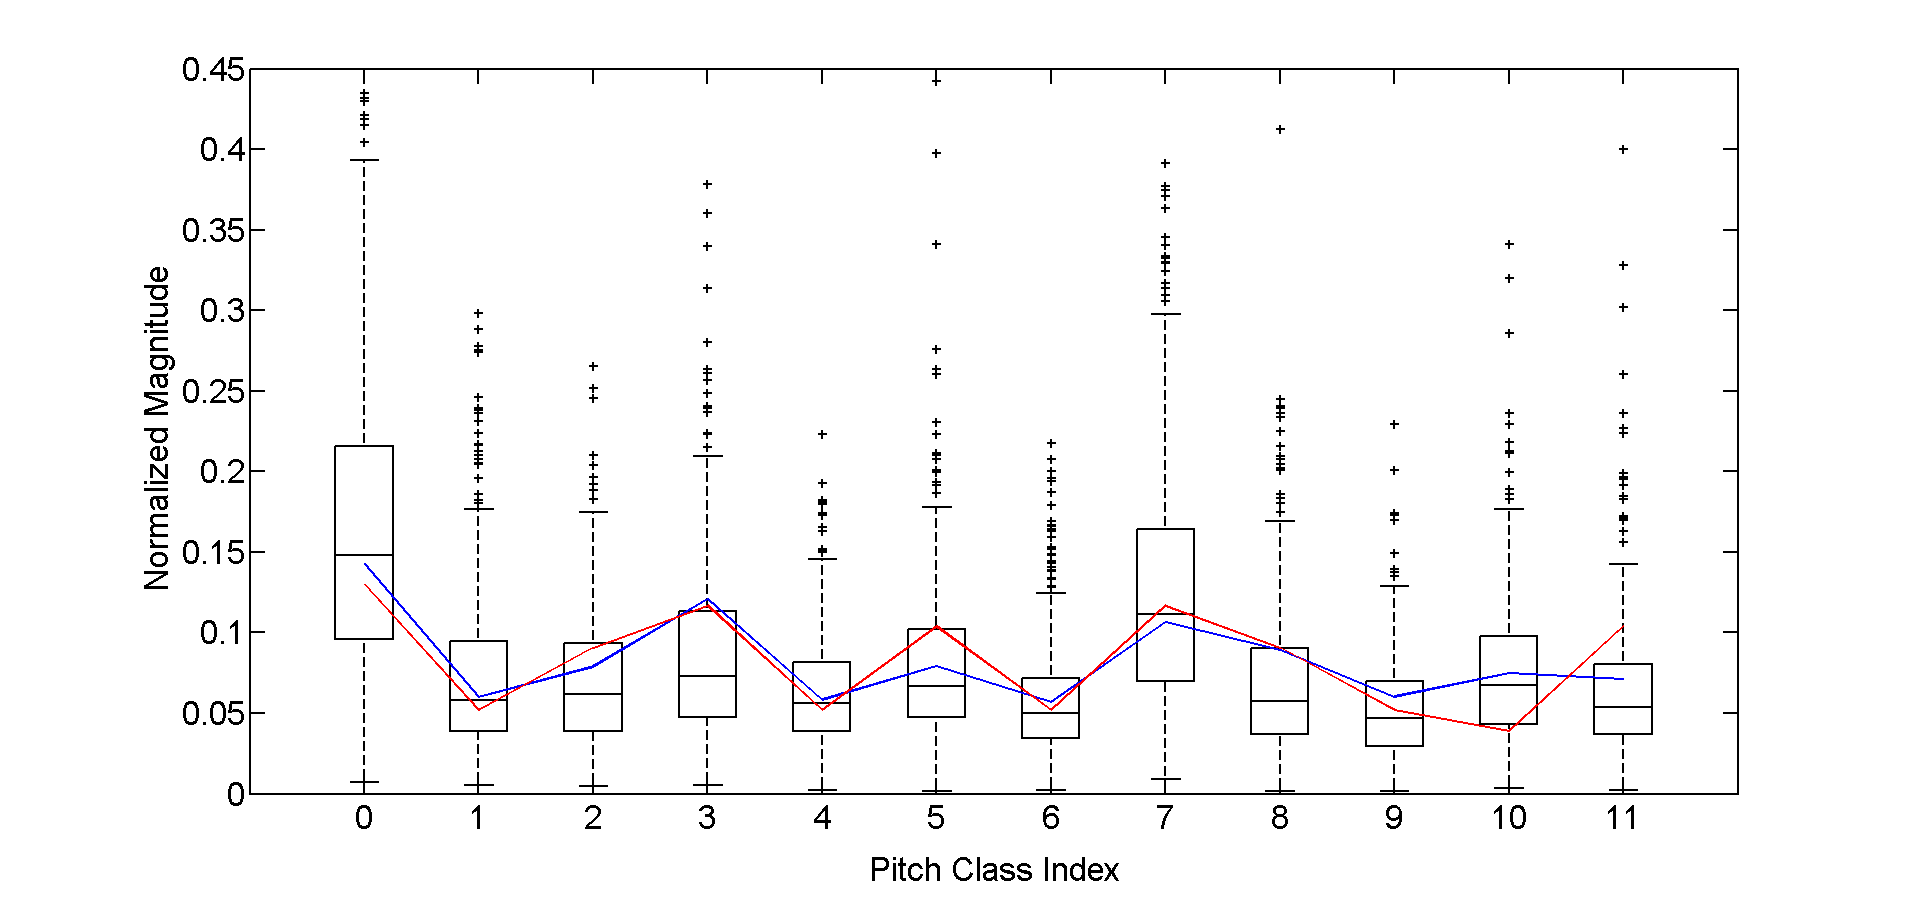
\includegraphics[scale=.2]{graph/allMinChroma+Krum+Temp}
	\caption{Major (left) and minor (right) key profiles for the complete data set, in comparison with two widely-used key profiles (Krumhansl in red and Temperley in blue).}
	\label{fig:OverallKeyProfiles}
\end{figure*}

\subsection{Genre-specific key profiles}
The key profiles of the six most populated genres are plotted in Fig.~\ref{fig:SpecificKeyProfiles}.
\begin{figure*}[tb]
    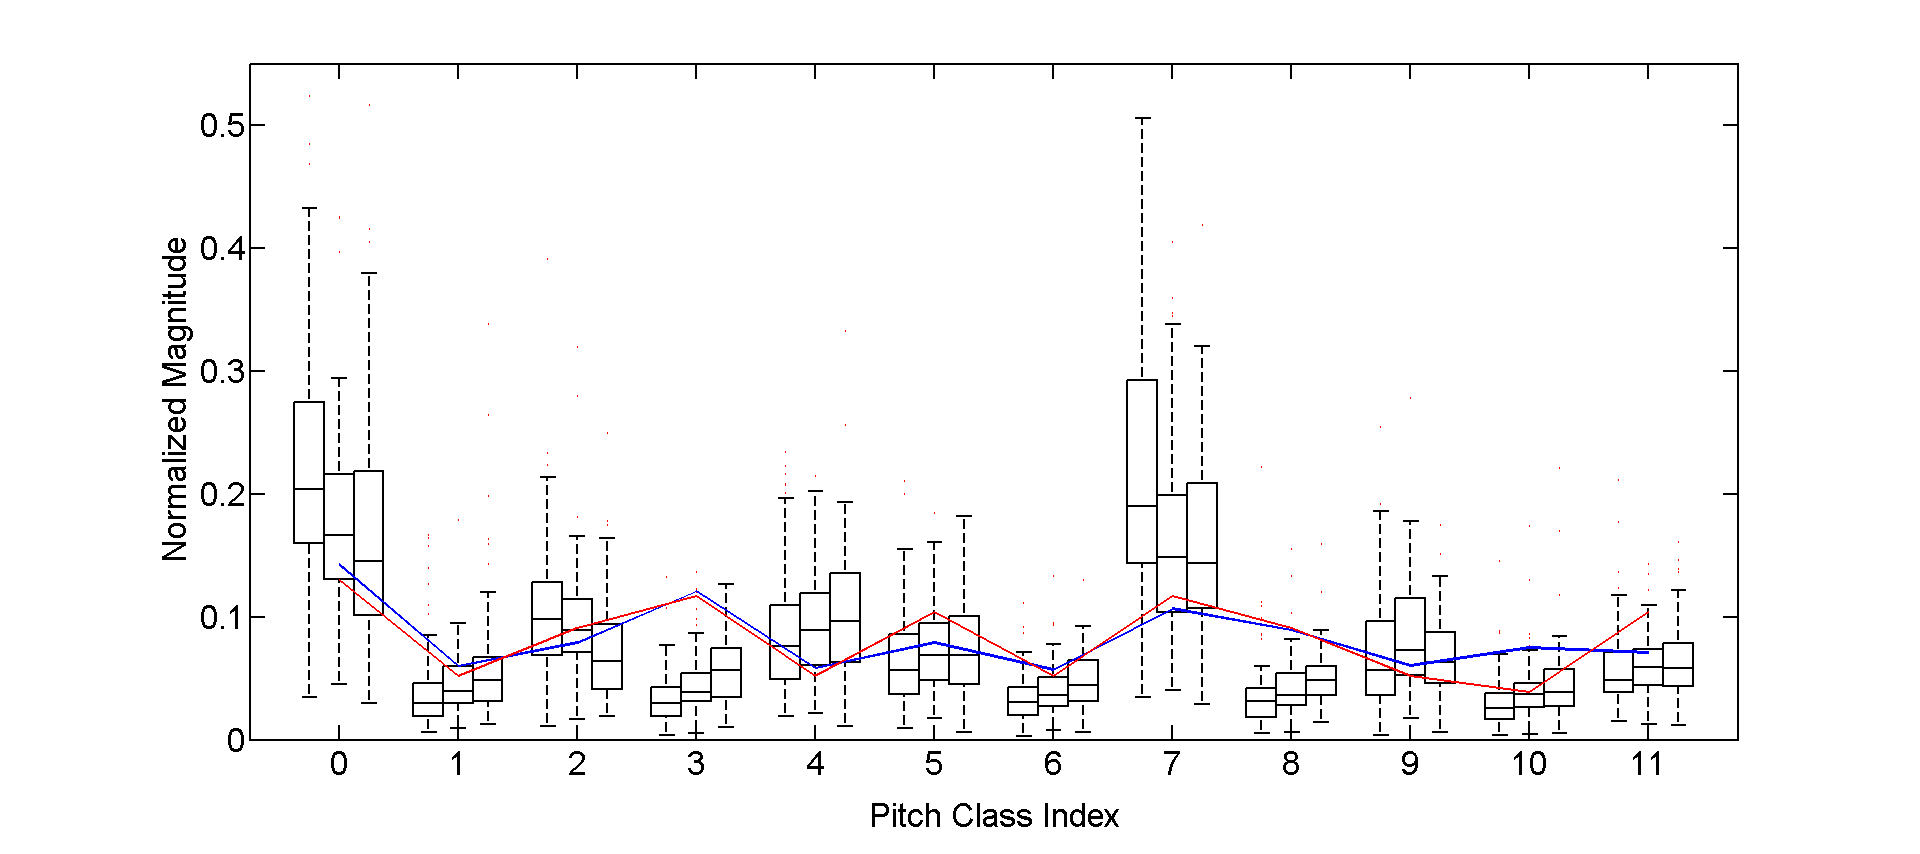
\includegraphics[scale=.2]{graph/boxPlotsMajCPR+Krum+Temp}
    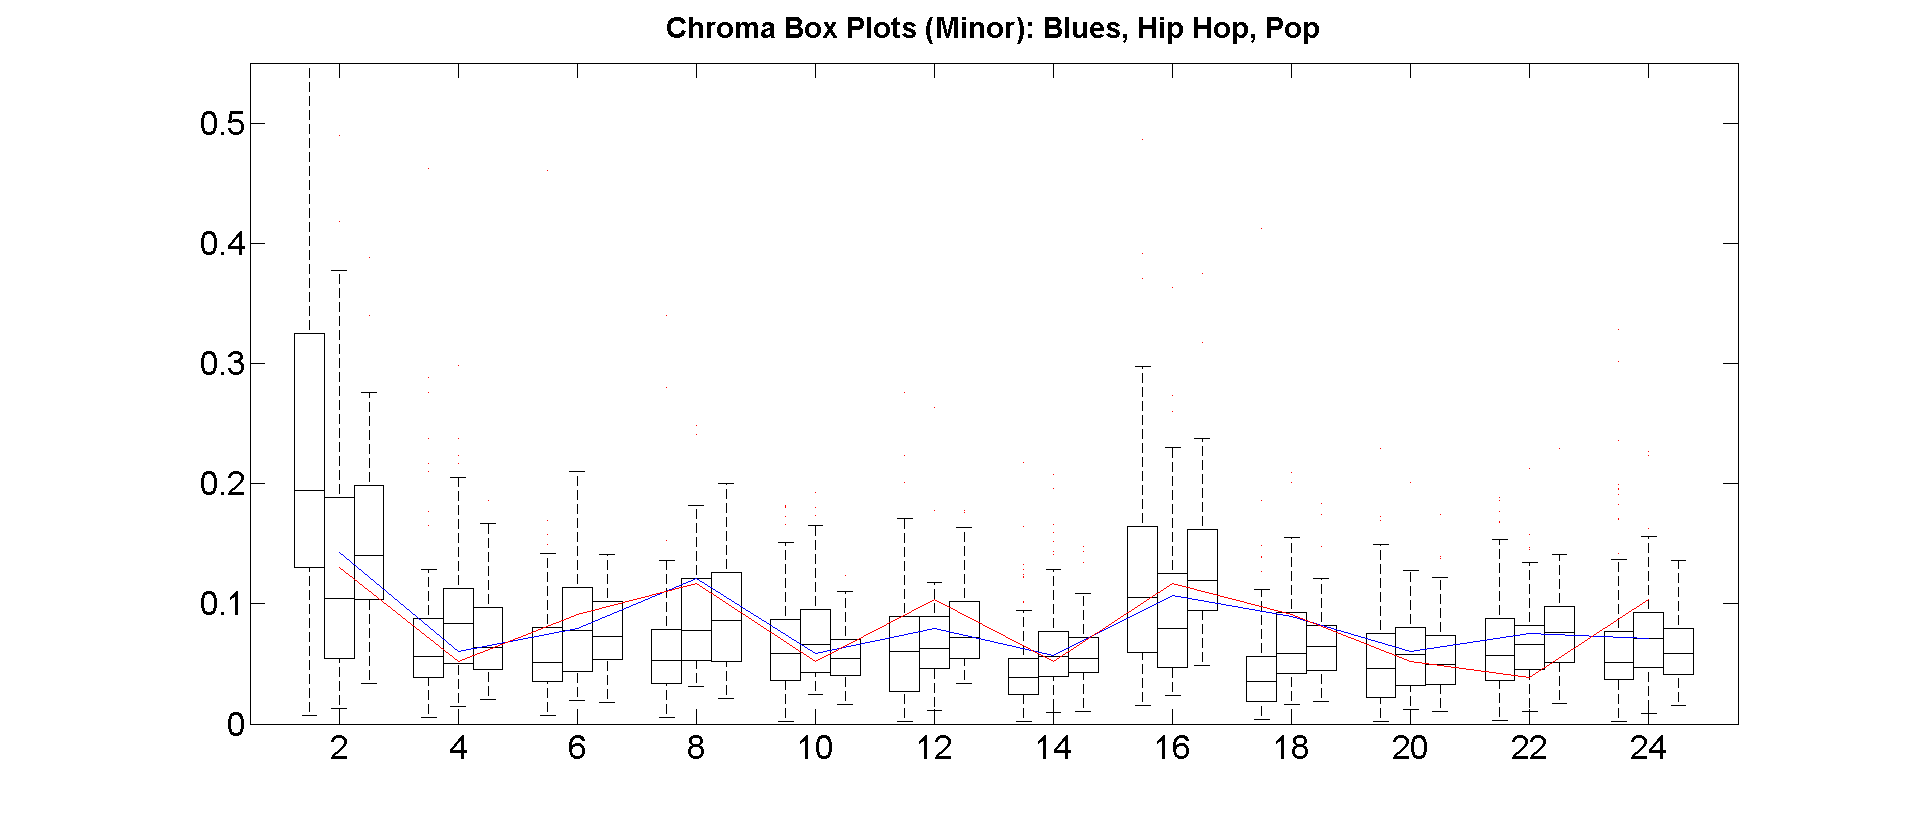
\includegraphics[scale=.2]{graph/boxPlotsMinBHP+Krum+Temp}
    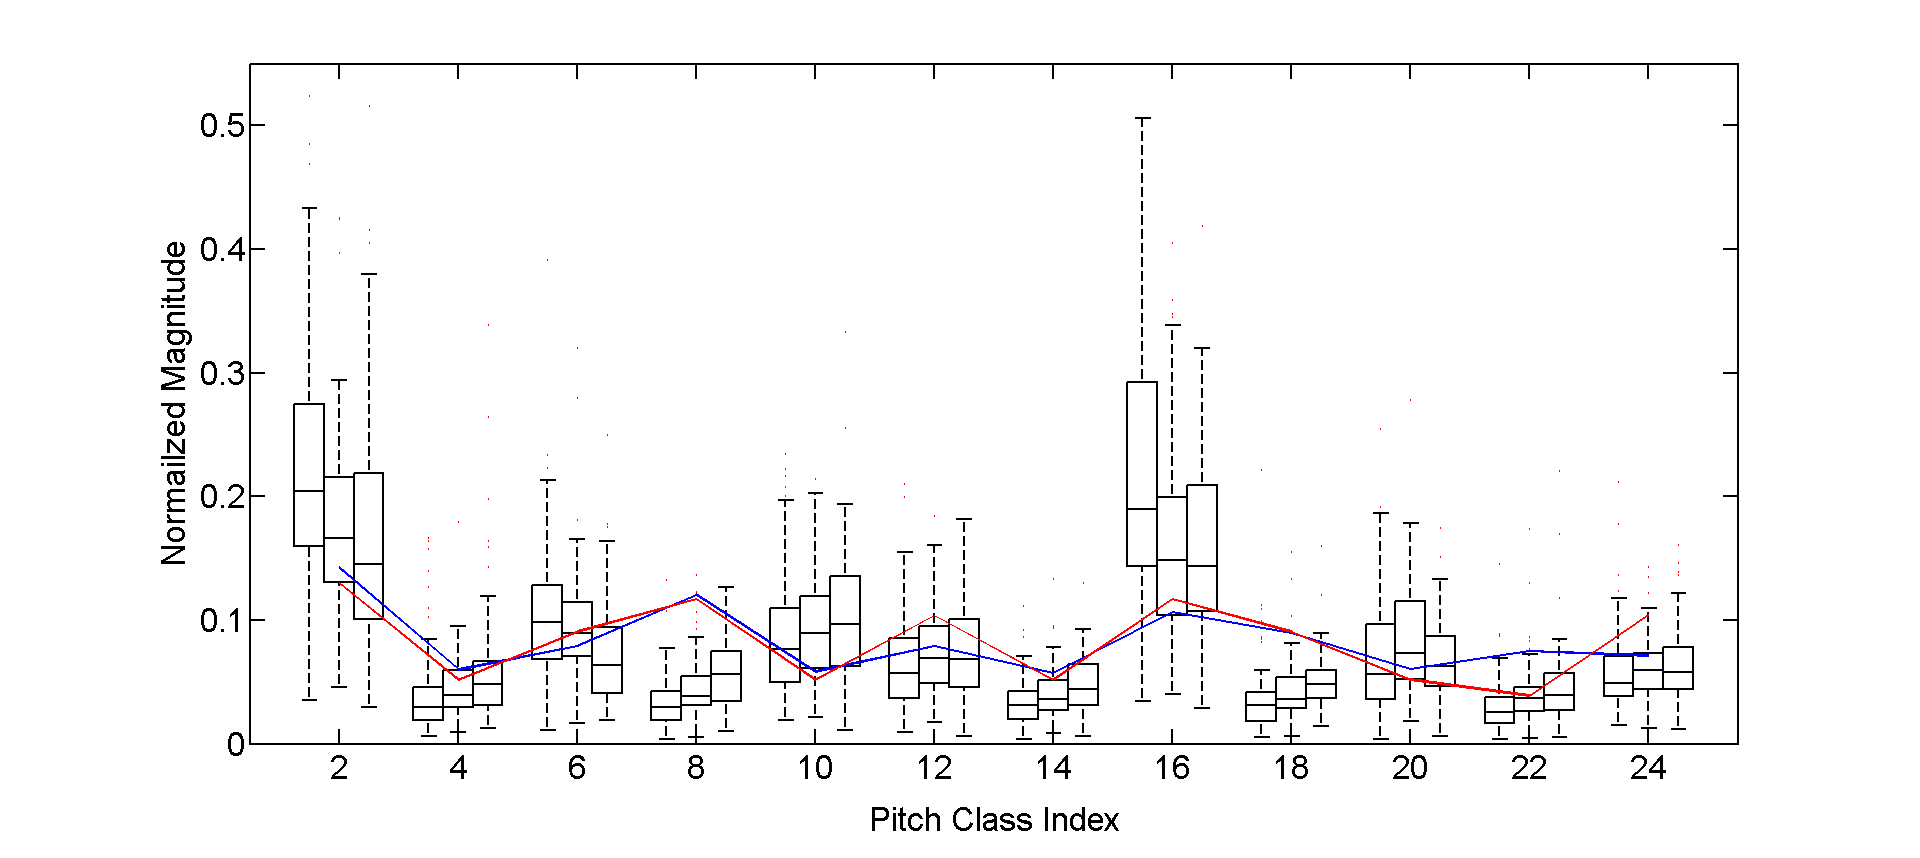
\includegraphics[scale=.2]{graph/boxPlotsMajDJRk+Krum+Temp}
    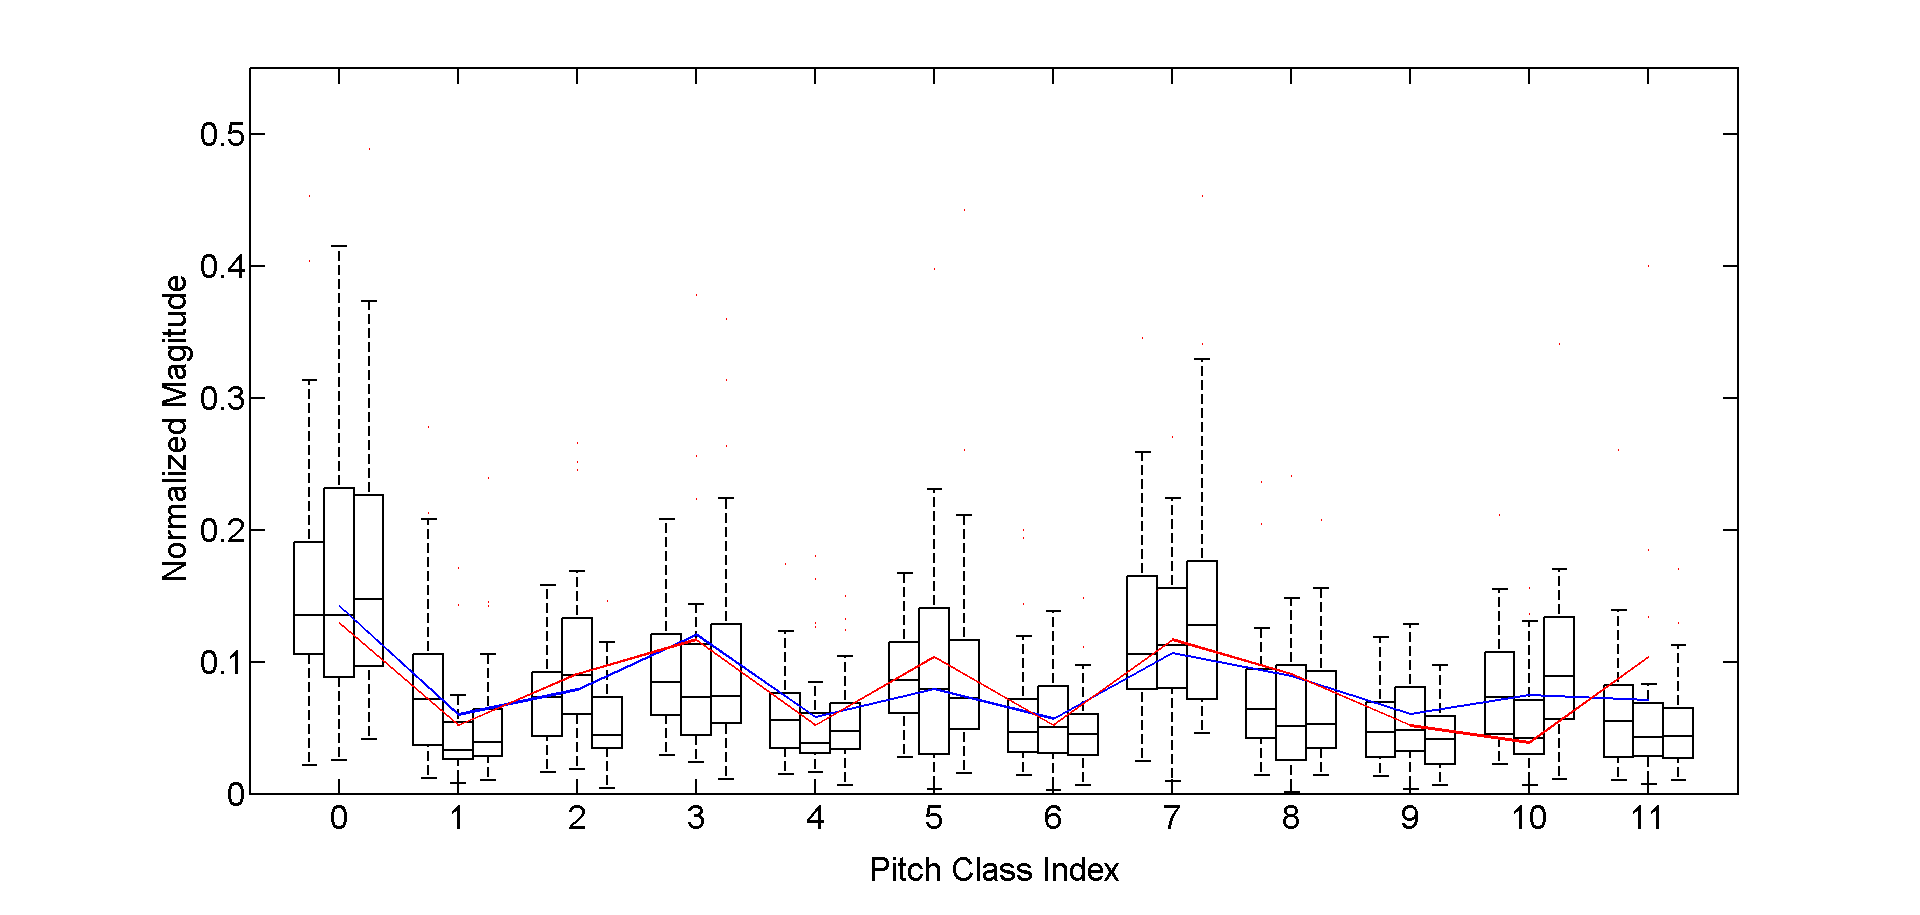
\includegraphics[scale=.2]{graph/boxPlotsMinDMR+Krum+Temp}
	\caption{Major (left) and minor (right) key profiles for the various genres, in comparison with the Krumhansl and Temperley profiles. SHOULD ALL 6 BE ONE FIGURE? I DON'T KNOW WHY THE ALIGNMENT IS WRONG HERE...}
	\label{fig:SpecificKeyProfiles}
\end{figure*}
The major distribution exhibits mostly a similar pattern with prominent spikes at the root note and the fifth. The Jazz distribution is one example that is noticeably different: it is rather flat and more uniform than the distributions of other genre's. It is to be expected that Jazz shows a wider range of pitches and harmonies and thus a more uniform pitch class distribution.

The distributions for minor have, compared to the major distributions, less distinct minima for non-scale pitches; especially the Blues distribution is ---~with the exception of root note and fifth~--- basically flat.

\subsection{Inter-genre distances}
In order to evaluate how distinct genres are with respect to their key profile, distance between all profiles were calculated using the Manhattan distance as shown in Tables~\ref{tab:GenreDistancesMajor} and \ref{tab:GenreDistancesMinor}. Genres for which the number of examples were less than 30 are grayed out. The labels are as follows: B is blues, C country, D disco, H hip-hop, J jazz, M metal, P pop, Rg Reggae, Rk is rock, K is the Krumhansl key profile, T the Temperley profile \cite{temperley_tonal_2007} and finally the overall median major/minor pitch profiles are denoted by Mdn.
\begin{table}
\centering
\resizebox{\columnwidth}{!}{%
        \begin{tabular}{|c||c|c|c|c|c|c|c|c|c||c|c|c|}
        \hline
        \textbf{Genre} &\ \textbf{B} & \ \textbf{C }& \ \textbf{D} & \ \textbf{H} & \ \textbf{J} & \ \textbf{M} & \ \textbf{P} & \ \textbf{Rg} & \ \textbf{R} & \ \textbf{Kr} & \ \textbf{Tp}  & \ \textbf{Mdn}\\
        \hline\hline
        \textbf{B}		 &0    &0.35    &0.40    &0.68    &0.44    &0.34    &0.35    &0.43    &0.31    &0.51    &0.59    &0.33\\
        \hline
        \textbf{C}  &0.35         &0    &0.27    &0.60    &0.32    &0.32    &0.17    &0.34    &0.20    &0.41    &0.47    &0.19\\
        \hline
        \textbf{D} 	&0.40    &0.27         &0    &0.33    &0.12    &0.21    &0.11    &0.12    &0.11    &0.15    &0.25    &0.09\\
        \hline
        \textbf{H} 	&0.68    &0.60    &0.33         &0    &0.27    &0.41    &0.42    &0.28    &0.43    &0.24    &0.29    &0.40\\
        \hline
        \textbf{J} 		&0.44    &0.32    &0.12    &0.27         &0    &0.25    &0.15    &0.17    &0.17    &0.12    &0.24    &0.13\\
        \hline
        \textbf{M} 	&0.34    &0.32   &0.21    &0.41    &0.25         &0    &0.20    &0.21    &0.16    &0.27    &0.41    &0.19\\
        \hline
        \textbf{P} 		&0.35    &0.17    &0.11    &0.42    &0.15    &0.20         &0    &0.19    &0.08    &0.23    &0.29    &0.05\\
        \hline
        \textbf{Rg} 	&0.43    &0.34    &0.12    &0.28    &0.17    &0.21    &0.19         &0    &0.17    &0.13    &0.23    &0.17\\
        \hline
        \textbf{R} 		&0.31    &0.20   &0.10    &0.43    &0.17    &0.16    &0.08    &0.17         &0    &0.23   &0.30    &0.06\\
        \hline\hline
				\textbf{Kr} 		&0.51    &0.41   &0.15    &0.24    &0.14    &0.27    &0.23    &0.13    &0.23         &0    &0.15    &0.21\\
				\hline
				\textbf{Tp}		&0.59   &0.47    &0.25    &0.29    &0.24    &0.41    &0.29    &0.23    &0.30    &0.15         &0    &0.28\\
				\hline
				\textbf{Mdn} 		&0.33    &0.19    &0.09    &0.40    &0.13    &0.19    &0.05    &0.17    &0.06    &0.21    &0.28         &0\\
				\hline
        \end{tabular}%
}
    
   
	\caption{Genre Distances for Major tracks using L1-norm}
	\label{tab:GenreDistancesMajor}
\end{table}

\begin{table}
\centering
\resizebox{\columnwidth}{!}{%
        \begin{tabular}{|c||c|c|c|c|c|c|c|c|c||c|c|c|}
        \hline
        \textbf{Genre} &\ \textbf{B} & \ \textbf{C }& \ \textbf{D} & \ \textbf{H} & \ \textbf{J} & \ \textbf{M} & \ \textbf{P} & \ \textbf{Rg} & \ \textbf{R} & \ \textbf{Kr} & \ \textbf{Tp}  & \ \textbf{Mdn}\\
        \hline\hline
        \textbf{B}		 & 0    &0.29   &0.27   & 0.30   &0.27    &0.18    &0.22  &0.33    &0.28    &0.28    &0.39    &0.18\\
        \hline
        \textbf{C}  &0.29         &0    &0.46    &0.59   &0.36    &0.45    &0.43    &0.43    &0.36   &0.53    &0.53    &0.41\\
        \hline
        \textbf{D} 	&0.27    &0.46         &0    &0.17    &0.20    &0.16    &0.10    &0.15    &0.19    &0.14    &0.20    &0.12\\
        \hline
        \textbf{H} & 0.30    &0.59    &0.17         &0    &0.28    &0.21    &0.17    &0.23    &0.33    &0.17    &0.27    &0.18\\
        \hline
        \textbf{J} 		&0.27    &0.36    &0.20    &0.28         &0    &0.23    &0.16    &0.19    &0.16    &0.24    &0.27    &0.15\\
        \hline
        \textbf{M} 	& 0.18    &0.45    &0.16    &0.21    &0.23         &0    &0.13    &0.26    &0.20    &0.14    &0.31    &0.09\\
        \hline
        \textbf{P} 		&0.22    &0.43    &0.10    &0.17    &0.16    &0.13         &0    &0.15    &0.16    &0.13   &0.25    &0.05\\
        \hline
        \textbf{Rg} 	&0.33    &0.43    &0.15    &0.23    &0.19    &0.26    &0.15         &0    &0.19    &0.18    &0.23    &0.18\\
        \hline
        \textbf{R} 		&0.28   &0.36    &0.19    &0.33    &0.16    &0.20    &0.16    &0.19         &0    &0.25    &0.33    &0.15\\
        \hline\hline
				\textbf{Kr} 		&0.28    &0.53    &0.14    &0.17    &0.24    &0.18    &0.13    &0.18    &0.25         &0    &0.16    &0.16\\
				\hline
				\textbf{Tp} 		& 0.39    &0.53    &0.20    &0.27    &0.27    &0.31    &0.25    &0.23    &0.33    &0.16         &0    &0.28\\
				\hline
				\textbf{Mdn} 		&0.18    &0.41    &0.12    &0.18    &0.15    &0.09    &0.05    &0.18    &0.15    &0.16    &0.28         &0\\
				\hline
        \end{tabular}%
}
   
	\caption{Genre Distances for Minor tracks using L1-norm}
	\label{tab:GenreDistancesMinor}
\end{table}
MAYBE IT's WORTH LOOKING AT A MATRIX THAT COMBINES THESE RESULTS? DID WE DECIDE TO THROW OUT THE MDS? I DON't REMEMBER.
CIAN-I DONT THINK WE MADE A DECISION EITHER WAY. I THINK MAYBE WE SHOULD INCLUDE ONE OR THE OTHER SINCE THEY BOTH CONTAIN ROUGHLY THE SAME INFORMATION?

Looking at the distance matrices, we can see that for major keys, the most similar genres are Rock and Pop while the most mutually distinct genres when considering major tracks are Country and Jazz. For minor tracks, Reggae and Pop are the most similar while Reggae and Rock are the most distinct.

Overall, Country and Jazz (major), and Blues (minor) are on average most dissimilar to all other genres (as well as the two template profiles), 

\section{Classification}
Musical genre recognition is a well studied field in MIR \cite{fu_survey_2011}. The most widely and successfully used features in this area are timbre features such as Mel Frequency Cepstral Coefficients (MFCC). MFCC seem well suited to picking up on instrumental and timbral differences between genres, although they are not totally independent of harmonic and tonal properties \cite{li_genre_2011}.
While the distance results indicate what genres are most similar and dissimilar, it does not allow an interpretation as to whether the genres distances do actually help to separate genres. In order to investigate how separable  our genre-specific key profiles are, we train an SVM classifier with our features (see Sect.~\ref{sec:featureset}) and compare the results with an MFCC-based classifier. The MFCC were calculated according to REFXXX: WHAT COMPUTATION DID YOU USE?. The mean and standard deviation of $12$ MFCC form a $24$-dimensional timbre feature vector.We used libSVM  \cite{chang_libsvm:_2011} and picked the SVM parameters with a grid search and 5-fold cross validation on a separate stratified split of the data. The classification is carried out for the $9$ classes described above.

While the KP1 feature (shifted by ground truth) are sufficient to prove or disprove separability, they can not used in a general classification scenario, as there will be no key label available. Therefore we also tested the following approaches to estimating a key-independent representation:
\begin{itemize}
    \item   \textbf{KP0: Unshifted}\\
        The overall pitch chroma of each song is used as extracted.
    \item   \textbf{KP1: Transposition by max}\\
        The overall pitch chroma of each song is shifted by the index of the maximum of this pitch chroma. Detecting the index of the maximum can be interpreted as the simplest possible root note estimation.
    \item   \textbf{KP2: Fourier transform}\\
        The shift dependent on the root note can be understood as the phase of the pitch chroma. The magnitude spectrum of the extracted pitch chroma is thus a phase-independent (and therefore root-note independent) representation. MAYBE IT MAKES SENSE TO RESORT THE PITCH CLASSES LIKE YOU DID IN YOUR KEY DISTRIBUTION PLOT BEFORE THE FFT?? %Firstly, for a given pitch chroma vector the mean over all bins is calculated and is subtracted from each component. 
    \item   \textbf{KP3: Transposition by ground truth}\\
        The overall pitch chroma of each song is shifted by the root note index annotated in the ground truth.
\end{itemize}

We investigated 3 classification scenarios: (i) only major keys, (ii) only minor keys, and (iii) the whole key-labeled data set without any differentiation between major and minor. All scenarios were carried out with the individual key profile features as well as with the combination of MFCCs and these features. The presented results are computed with 10-fold cross validation.
The overall range of results is consistent with the results of Tzanetakis and Cook, who ---~ for the complete set with 10 classes (i.e., including the ambiguous samples) using a GMM classifier~--- reported a 23\% classification accuracy for a set of simple pitch histogram features and a 47\% accuracy for 10 MFCC \cite{tzanetakis_musical_2002}. 


%As with any classification task, the feature used to summarize tracks is an important concern. Previous work in this area has shown that timbral features, particularly Mel Frequency Spectrum Coefficients, are especially suited to the task of predicting genre. While MFCC are suited to picking up on instrumental and timbral difference between genres, some work has shown that they are not totally independent of harmonic or tonal information \cite{li_genre_2011}. Here we investigate the extent to which tonal information can be used to discern genres y examining the distributions of pitch chroma within each of 9 different genres. First we examine the overall distribution of keys for each genre. Next different methods for transposing pitch chroma to a key-independent representation are introduced and we look at the chroma distributions using chroma box plots, inter-genre distance and mulch-dimensional scaling. In the final section we test the degree to which the chroma distribution separate gen-res by performing classification with an SVM using chroma and combined chroma/MFCC features.


%To investigate this effect, we train and evaluate a Support Vector Machine using libSVM \cite{chang_libsvm:_2011}.
%The SVM hyper-parameters (C, \gamma) representing the margin and kernel widths were tuned using a grid-search and 5-fold cross validation on a separate stratified split of the data (I HAVE NO IDEA WHAT THAT MEANS). Best performance was achieved using a non-linear SVM with Radial Basis Function kernel.
%We investigated the following scenarios: (i) the whole key-labeled data set with no differentiation between major and minor and (ii) the major/minor subsets individually in order to control for the differences in major/minor distribution between keys. 
%10-fold cross validation  accuracy was calculated using the raw pitch chroma, max-shifted key profile, the Fourier pitch chroma and the key profile shifted according to the ground truth. We compare the results to a classifier based on a set of MFCC features as well as a combination of MFCC and key profile features. MFCC features were calculated according to REFXXX: WHAT COMPUTATION DID YOU USE?. The mean and standard deviation of $12$ MFCCs form a $24$-dimensional timbre feature vector. %as follows: for each block we compute 12 MFCC coefficients, then take the mean and standard deviation over the whole song. These features are then concatenated to form a 24 dimensional feature vector.

Table~\ref{tab:accuracyPC} summarizes the results of the SVM classification for the different key profile computations, and Tab.~\ref{tab:accuracyPC+MFCC} shows the mode-independent results when combined with the MFCC features. LET'S MAKE ONE BIG TABLE AND ALSO CALCULATE ALL THE MFCC-RELATED VALUES FOR MAJOR AND MINOR AS WELL. ALSO RENAME THE FEATURES TO KPX. AND WE NEED THE ZEROR CLASSIFIER.
\begin{table}
\begin{center}
    \begin{tabular}{|l|l|l|l|}
      \hline 
	\bf Feature & \bf Major & \bf Minor & \bf All\\
	\hline
	KP0 & 35.35 ± 2.53 & 37.90 ± 1.39 & 35.04 ± 1.97\\
	\hline
	KP1 & 37.24 ± 2.35 & 34.72 ± 2.21 & 35.91 ± 1.65\\
	\hline
	KP2 & 37.74 ± 2.29 & 36.36 ± 2.58 & 32.36 ± 2.08\\
	\hline
	KP3 & 40.33 ± 2.04 & 39.66 ± 3.33 & 33.83 ± 0.92\\
 	\hline

    \end{tabular}
    \caption{Classification accuracy for different key profile computations.}
    \label{tab:accuracyPC}
  \end{center}
\end{table}

\begin{table}
\begin{center}
    \begin{tabular}{|l|l|}
      \hline 
	\bf Feature & \bf Accuracy\\
	\hline
	MFCC & 55.01 ± 2.96\\
	\hline
	MFCC+KP01 & 59.31 ± 2.08\\
	\hline
	MFCC+KP1 & 59.14 ± 1.70\\
	\hline
	MFCC+KP2 & 57.93 ± 1.66\\
 	\hline
	MFCC+KP3 & 59.94 ± 2.02\\
 	\hline

    \end{tabular}
    \caption{Classification accuracy for different key profile computations in cobmbination with MFCC features.}
    \label{tab:accuracyPC+MFCC}
  \end{center}
\end{table}

%MAYBE INCLUDE A 'BASELINE' CLASSIFICATION BASED ONLY ON THE KEY (NOT THE PITCH CHROMA) HERE FOR COMPARISON???

Figures \ref{fig:confMatMajPC}, \ref{fig:confMatMinPC}, and \ref{fig:confPC+MFCC} display the confusion matrices of the classification results. PLEASE ADD ANOTHER ROW TO THE MATRICES WITH THE SUM OVER COLS - WE HAVE TO REDO ALL OF THESE ANYWAY, WE DONT WANT THEM AS PNGs.
\begin{figure}[tb]
    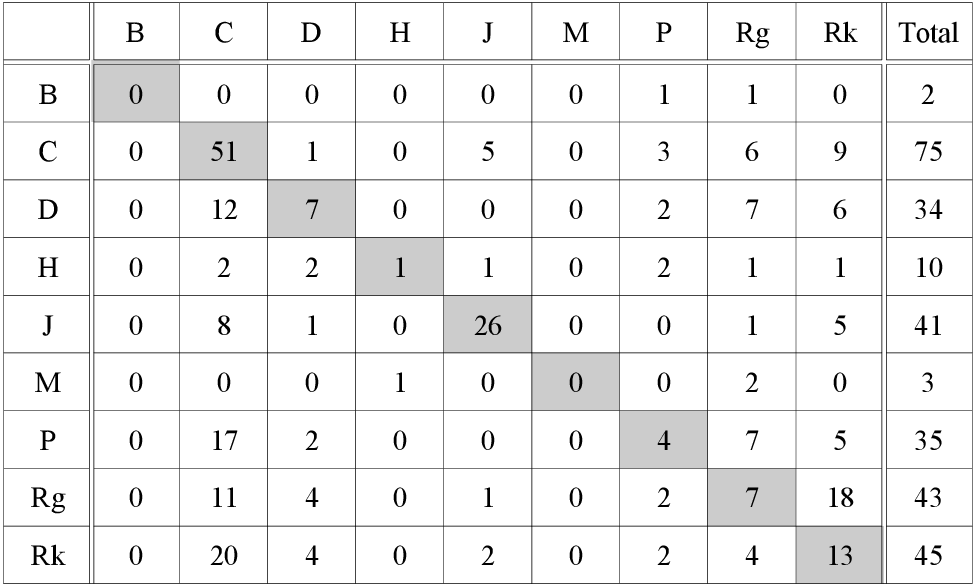
\includegraphics[scale=.4]{graph/confMatMajPC}
	\caption{CONFUSION MATRIX 1, major}
	\label{fig:confMatMajPC}
\end{figure}
\begin{figure}[tb]
    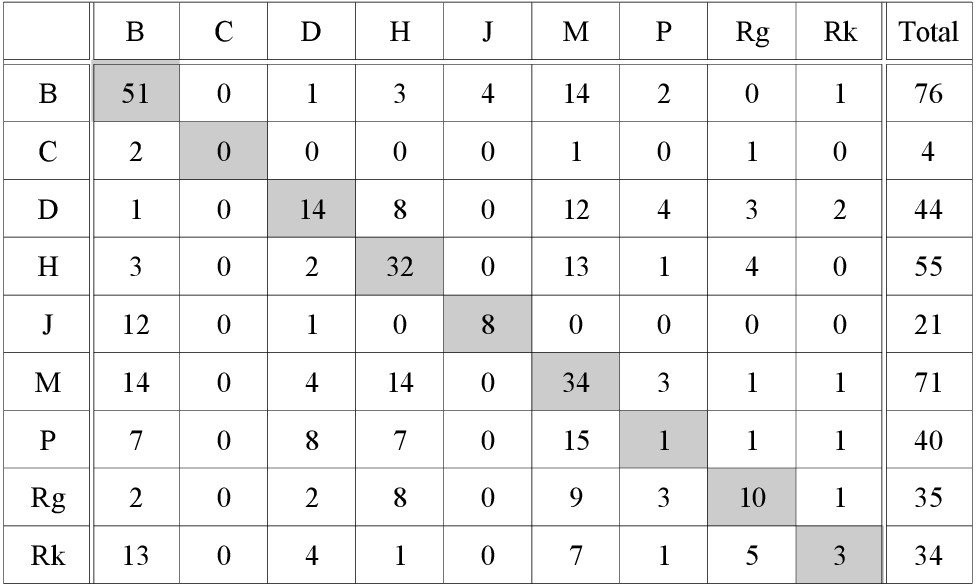
\includegraphics[scale=.4]{graph/confMatMinPC}
	\caption{CONFUSION MATRIX 2, minor}
	\label{fig:confMatMinPC}
\end{figure}
\begin{figure}[tb]
    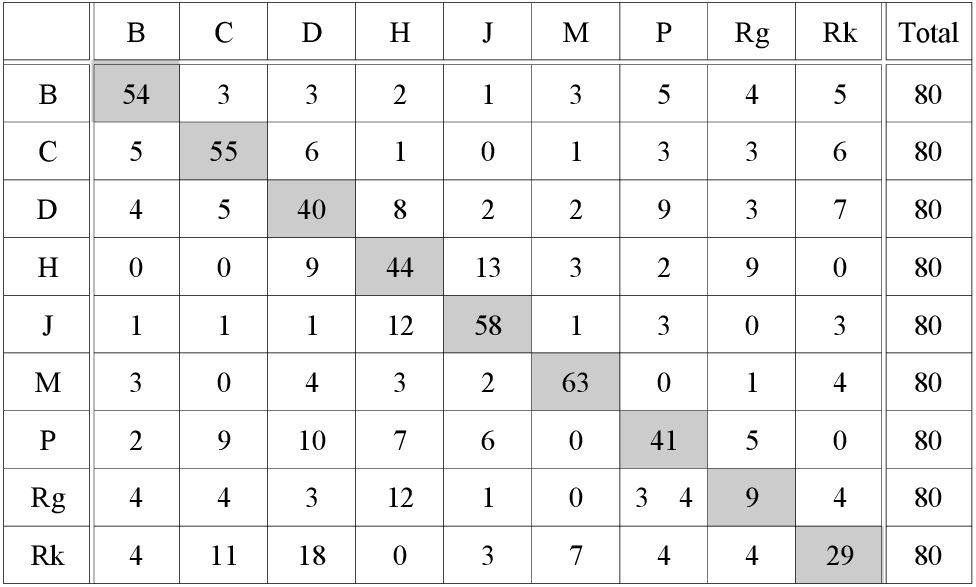
\includegraphics[scale=.4]{graph/confPC+MFCC}
	\caption{CONFUSION MATRIX 3, pc + mfcc}
	\label{fig:confPC+MFCC}
\end{figure}
DESCRIBE AND DISCUSS ME.

\subsection{Results and discussion}
\begin{itemize}
    \item   table: profile-based classification worse than timbre classification
    \item   table: ground truth shifting better than other features, except when combining modes
    \item   table: FFT shift in the same range as Max shift
    \item   table: unshifted not much worse than shifted
    \item   major confusion matrix: many classifications into country, minor confusion matrix: many classifications into  metal --- why?
\end{itemize}
COULD YOU ALSO GENERATE THE NORMALIZED CONFUSION MATRICES, SO THAT THE ACCURACY PER CLASS IS ON THE DIAGONAL? I DON'T WANT TO ADD THEM TO THE PAPER< I JUST WANT TO LOOK - MAYBE THERE IS SOMETHING MORE EVIDENT THAN WITH THE ABSOLUTE NUMBERS.

One fact revealed in this analysis is the relatively small performance increase observed by sorting the chroma, even when using the ground truth directly. By sorting the chroma any information on the genre given by the key has been removed (for example as a prior estimate based on the key distributions in each genre) which would, it is hoped, reveal any differences in the distributions. 
However, whether or not this technique improves performance depends on the initial distribution of pitch chroma; suppose genre groups are perfectly separable given their key-independent chroma distributions and then for each song we transpose it into a new key with some related probability. Since cyclic-transpositions correspond to reflections this process is unlikely to make the data significantly more or less separable, which may explain the small in-crease in performance when using sorted chroma. I STILL CANNOT FOLLOW HERE!
Splitting the data into major and minor results in slightly improved accuracy, however in this case we have added information by using the ground truth and realistically harmony estimation should be done automatically which would be an additional source of error.
	Unsurprisingly MFCCs vastly outperformed pitch chroma features alone. However, combining features results in a slight performance increase in overall accuracy of around 4-5\% indicating that the pitch chro-ma distributions contain at least some genre-relevant information.
    
    FROM THE OVERALL PROFILE SECTION ABOUT JAZZ: This agrees with the classification results of Section 5, where Jazz was one of the least confused major genres.
    
    MENTION RANDOM CLASSIFICATION RATE - SHOULD BE AROUND 11\%, but we have nonuniform class distributions. ZeroR classifier?
    
    LETS NOT FORGET THAT WE DO NOT ACTUALLY WANT TO CLASSIFY, WE JUST WANT TO SHOW THAT THE GENRES ARE SEPARABLE WRT THEIR KEY PROFILE.
    
    DISCUSS CONFUSION MATRICES

\section{Conclusion}
\begin{itemize}
    \item   some genres are separable, but overall the similarities between the key profiles outweigh the differences
    \item   mention most similar and most separate genres
    \item   not a proposal to use these profiles but to investigate whether there are genre dependent differences or not.
\end{itemize}


\bibliography{ChromaPaper}

\end{document}
